\chapter{\SM}

El {\SM} de la física de altas energías (SM) describe correctamente a los
constituyentes de la materia y sus interacciones. Esta teoría fue formulada en
varios trabajos a partir de la segunda mitad del siglo XX y prácticamente todos
los datos obtenidos con los experimentos de altas energías pueden explicarse
dentro de este marco. Sin embargo este modelo tiene algunas debilidades tanto
teóricas como experimentales y por lo tanto no puede ser considerado como una
teoría fundamental.

En este capítulo se describe brevemente las características mas relevantes de
esta teoría y al final se detallan algunas de las debilidades que dan lugar a
los modelos que intentan explicar la física mas allá del SM.


\section{Las partículas fundamentales y sus interacciones}

De acuerdo al SM toda la materia esta compuesta por un número peque\~no de
partículas fundamentales de espín $1/2$, fermiones, que se
dividen en dos tipos: quarks y leptones (ver \cref{tab:fermions}). Hasta el
momento, ningún experimento ha podido encontrar evidencia de que estos fermiones
tengan una subestructura interna. Los quarks y leptones además están divididos
en tres generaciones o familias, ordenadas según su masa. Como las partículas
de las generaciones mas altas tienen mayor masa y son inestables decaen
en partículas de generaciones mas bajas. Es por este motivo que la materia
ordinaria esta formada por partículas de la primer generación.

\begin{table}[!ht]
  \centering
  \begin{tabular}{cccccccc}
    \hline
    & \multicolumn{3}{c}{Partícula} & \multicolumn{3}{c}{Masa} & Carga Eléctrica \\

    \hline
    \multirow{2}{*}{Leptones}
    & e & $\mu$ &  $\tau$ & 511 \kev & 105.7 \mev & 1768 \mev & -1  \\
    & $\nu_e$ & $\nu_\mu$ & $\nu_\tau$ & $<2.2 \eV$ & $< 0.17 \mev$ & $<15.5 \mev$ & 0 \\
    \hline
    \multirow{2}{*}{Quarks}
    & $u$ & $c$ & $t$ & 2.4 \mev & 1.27 \gev & 171.2 \gev & 2/3 \\
    & $d$ & $s$ & $b$ & 4.8 \mev & 104 \mev & 4.2 \gev & -1/3 \\
    %\hline
  \end{tabular}
  \caption{Partículas fundamentales de materia del SM. Las tres columnas internas representan las
    tres generaciones, ordenadas segun su masa. En la segunda y tercer columna se encuentra
    la masa y la carga electrica, respectivamente. \hl{Mejorar tabla}}
  \label{tab:fermions}.
\end{table}

La distintas interacciones entre quarks y leptones son descriptas en el SM en términos del
intercambio de partículas entre estos. Estas partículas de intercambio son
los \emph{bosones} de gauge, y tienen espín entero.
Los bosones mediadores se muestran en la \cref{tab:bosons}.

Existen cuatro tipos de interacciones fundamentales. La interacción fuerte es la
responsable de mantener los quarks formando los protones, neutrones y hadrones en general, y es
mediada por partículas no masivas llamadas \emph{gluones}. Las interacciones
electromagnéticas son las responsables de todos los fenómenos extra nucleares,
como por ejemplo las fuerzas intermoleculares en líquidos y solidos. Estas
interacciones están mediadas por el intercambio de fotones no masivos. La
interacción débil es la responsable de los procesos de decaimiento $\beta$, y
sus mediadores son los bosones $Z^0$ y $W^\pm$, con masas del orden de 100 veces
la masa del protón. Por último existe una interacción que actúa entre todo tipo
de partículas masivas, la interacción gravitatoria. Actualmente no existe ninguna teoría
cuántica completa que explique esta interacción fundamental, aunque hay muchas
teorías propuestas que postulan la existencia de una partícula de espín 2 que
media la gravedad, denominada \emph{gravitón}. En la escala de los experimentos
de partículas es la interacción mas débil de todas las interacciones
fundamentales, aunque es la dominante en la escala del universo, \hl{y será despreciada
en lo que sigue}.

Los leptones interactúan de forma débil y electromagnética en el caso de ser
cargados, o solo débilmente si son neutros. En contraste, los quarks (que son
los constituyentes fermiónicos de los hadrones, y por lo tanto del núcleo
atómico) interactúan además de débil y electromagnéticamente, por medio de la
interacción fuerte. Esta es la distinción fundamental entre quarks y leptones.


\begin{table}[!ht]
  \centering
  \begin{tabular}{cccccccc}
    \hline
    Fuerza & Partícula & Masa \\
    \hline
    Débil    &   $W^\pm$ y $Z^0$ & 80.398 y 91.1876  \\ %%$\mu$ &  $\tau$ & 511 \kev & 105.7 \mev & 1768 \mev & -1  \\
    \hline
    Electromagnética & $\gamma$ & 0 \\
    \hline
    Fuerte & $g$ & 0\\
    \hline
  \end{tabular}

  %% \begin{tabular}{ccc}
  %%   \hline Débil &  & Fuerte \\
  %%   \hline quarks y leptones &  & quarks \\
  %%   \hline  & $\gamma$ & gluones \\
  %%   \hline
  %% \end{tabular}

  \caption{Interacciones y los bosones de gauge mediadores de las mismas.\hl{Mejorar tabla}}
  \label{tab:bosons}
\end{table}


\section{El \SM}

Formalmente, el {\SM} es una teoría cuántica de campos renormalizable que provee
una descripción de los campos que describen las partículas fundamentales, y las
interacciones fuerte, débil y electromagnética.
Estas interacciones surgen del requerimiento de que la teoría sea invariante
bajo transformaciones de gauge locales del grupo de simetría:

\begin{equation}
  \text{SU}(3)_C \times \text{SU}(2)_L \times \text{U}(1)_Y
\end{equation}
%
donde $Y$, la hipercarga, $L$, la helicidad izquierda, y $C$, la carga de color,
representan las cantidades conservadas del grupo de simetría. El subgrupo
$\text{SU}(2)_L \times \text{U}(1)_Y$ representa el sector electrodébil, es
decir, la electrodinámica cuántica (QED) mas las interacciones débiles.
%% La electrodinamica cuantica (QED) es una descripcion precisa
%% de las interacciones electromagneticas. Esta teoria fue una de
%% los logros mas importantes del siglo XX.

%% Es una teoria cuantica
%% de campos que conecta el formalismo moderno de la mecanica cuantica
%% con los principios clasicos del electromagnetismo. Uno de los
%% logros mas notables es el calculo preciso del momento magnetico
%% del electron, que acuerda con las medidas experimentales hasta
%% al menos los diez primeras cifras decimales. En QEDm la fuerza
%% entro dos particulas cargadas esta carazterizada por el itercambio
%% de un campo cuantico: el foton. En 1954 Yang and Robert Mills
%% formularon un principio general de invarianza de gauge}

Y la adición del grupo $\text{SU}(3)_C$ incluye la cromodinámica cuántica, que
es la teoría de campos de gauge que describe las interacciones fuertes de los
quarks y gluones que poseen carga de color.

La masa de las partículas en el SM puede ser introducida mediante el llamado
mecanismo de Brout-Englert-Higgs\cite{PhysRevLett.13.321, PhysRevLett.13.508}, vía la ruptura
espontánea de la simetría electrodébil.

\begin{equation}
  \text{SU}(3)_C \times \text{SU}(2)_L \times \text{U}(1)_Y \to \text{SU}(3)_C
  \times \text{U}(1)_Q
\end{equation}
%
que resulta en la generación de los bosones de gauge masivos $W^\pm$ y $Z$. Como
consecuencia de esto, además, un nuevo campo escalar debe ser agregado al
Lagrangiano, dando lugar a la aparición de un nuevo bosón masivo, $H$, de espín
0, al que se lo llamó \emph{bosón de Higgs}.

Weinberg y Salam fueron los primeros en aplicar el mecanismo de Higgs al
rompimiento de la simetría electrodébil
\cite{PhysRevLett.19.1264,PhysRev.127.965} y mostraron como este mecanismo podía
ser incorporado a la teoría electrodébil de Glashow \cite{Glashow1961579}, dando
inicios a lo que hoy conocemos como SM de la física de partículas.

La relación entre las masas de los bosones $W^\pm$ y $Z$ predicha por el SM esta
dada por $m_W/m_Z = \cos \theta_W$, donde $\theta_W$ es el ángulo de
mezcla de Weinberg, y relaciona la constante de acoplamiento débil ($g$) con la
electromagnética ($g'$) como $\tan\theta_W = g'/g$. Los bosones $W^\pm$ y $Z$
fueron descubiertos en 1982 por las colaboraciones UA1 y UA2 del experimento
SppS del CERN.

No sólo los bosones de gauge adquieren masa debido al mecanismo de Higgs,
también lo hacen los fermiones que forman la materia. El descubrimiento del
quark top en 1995 por las colaboraciones D0 y CDF, con una masa de $\sim 173
\GeV$, terminó por cerrar las partículas que conforman la materia.

Desde el punto de vista teórico la masa del bosón de Higgs es un parámetro libre
dentro del SM y por lo tanto ninguna predicción puede ser hecha. La búsqueda
del bosón de Higgs, la única partícula del SM que no había sido descubierta
aún, fue uno de los grandes objetivos por los cuales se dise\~no y construyó el
Gran Colisionar de Hadrones (LHC). En el a\~no 2012 el CERN anunció el
descubrimiento de una partícula consistente con el bosón de Higgs por parte de
los dos grandes experimentos del LHC, ATLAS y CMS
\cite{Aad:2012tfa,Chatrchyan:2012ufa}. La medición combinada entre ATLAS y CMS
de la masa del Higgs es $125.09 \pm 0.21 \text{(stat.)} \pm 0.11 \text{(sist.)}
\gev$. El descubrimiento del bosón de Higgs completó el espectro de partículas del SM.

\begin{figure}[!htbp]
  \centering 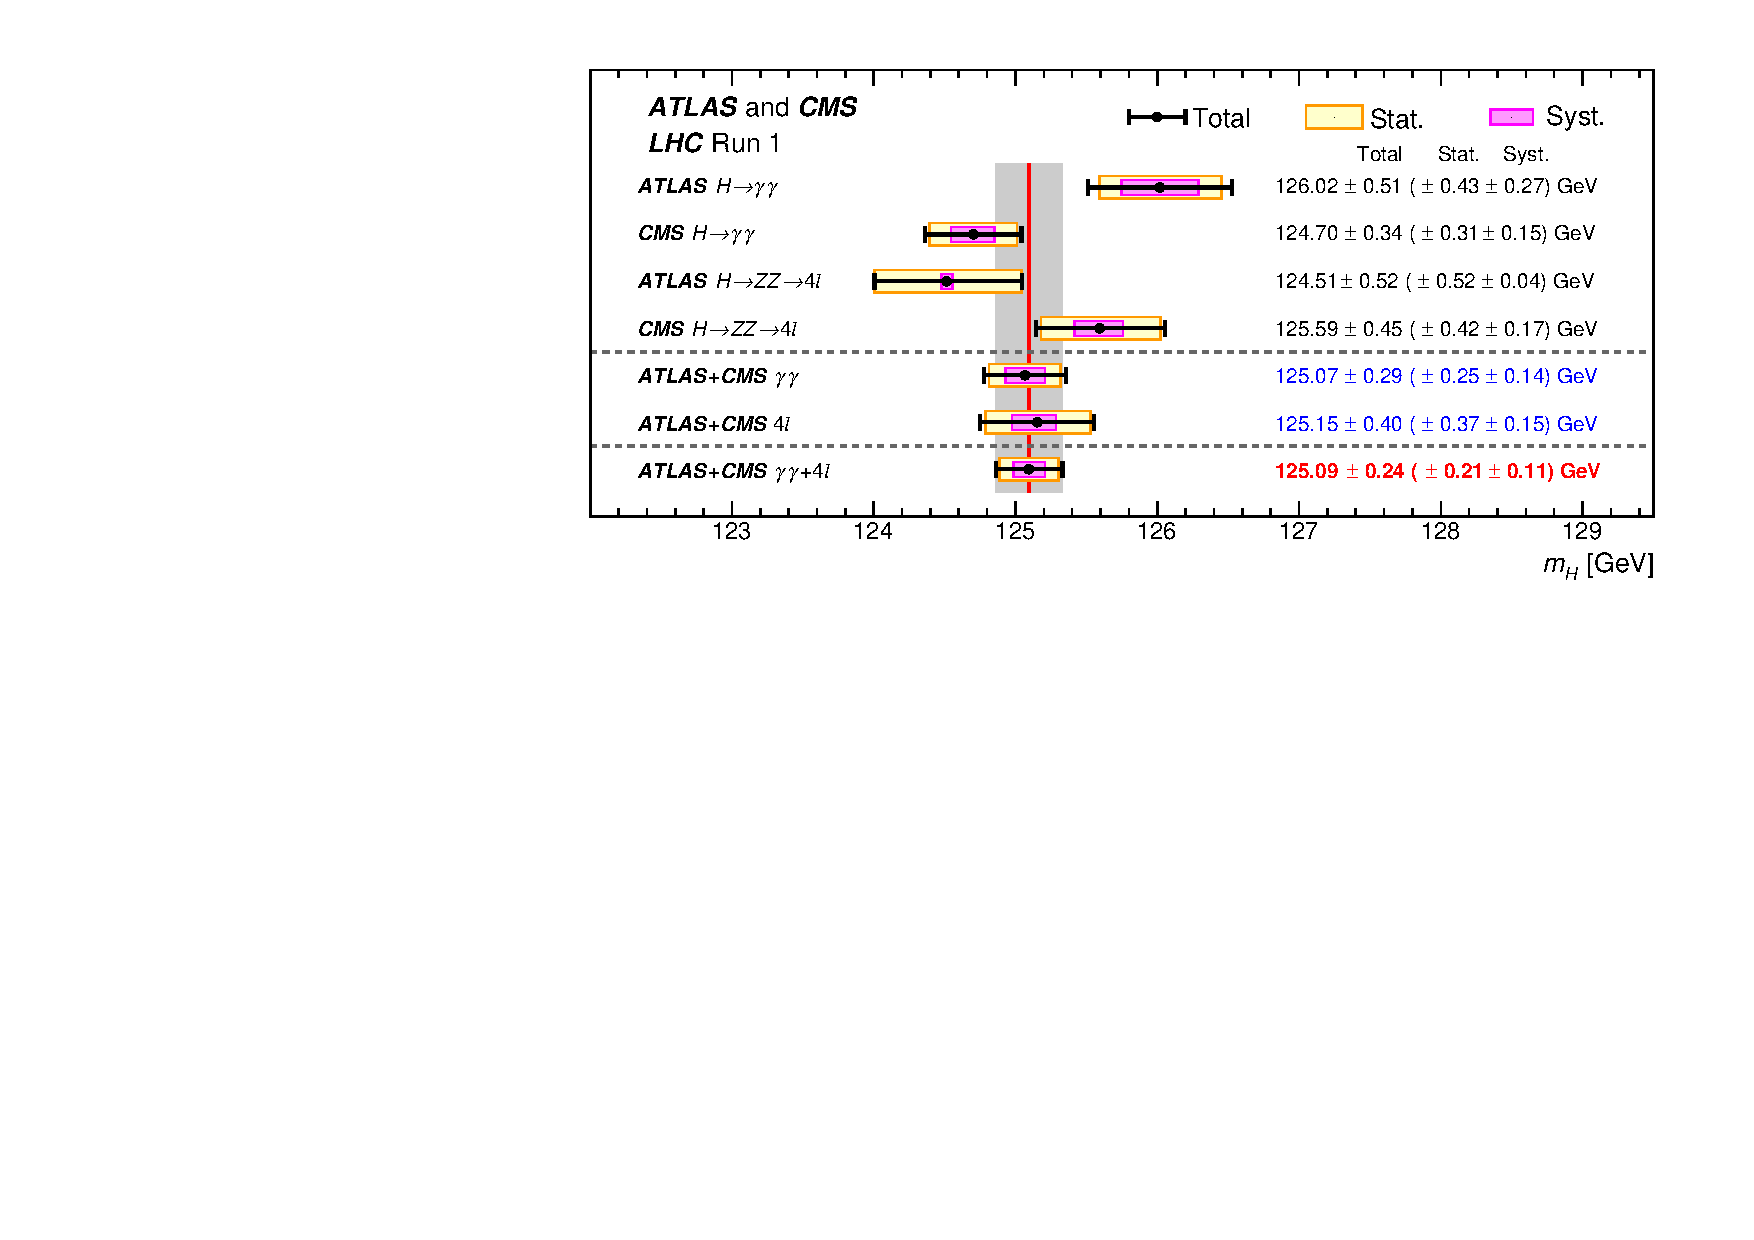
\includegraphics[width=0.8\textwidth]{figures/higgs_atlas_cms_mass}
  \caption{Resumen de las mediciones de la masa del bosón de Higgs de los
    distintos análisis de ATLAS y CMS, y del análisis combinado. Se indican las
    incertezas sistemáticas (bandas de color magenta), estadísticas (bandas de
    color amarillo), y total (bandas negras). La linea roja vertical y la
    correspondiente sombra gris indican el valor central y la incerteza total de
    la medida combinada, respectivamente\cite{HiggsMass_ATLAS_CMS}.}
  \label{fig:higgs_cms_atlas}
\end{figure}

Todas las observaciones experimentales son compatibles con el SM a un nivel de
muy alta precisión. La \cref{fig:sm_atlas_xs} muestra el buen acuerdo entre la
sección eficaz de algunos procesos del SM medidas por ATLAS y las predicciones
teóricas.

\begin{figure}[!htbp]
  \centering
  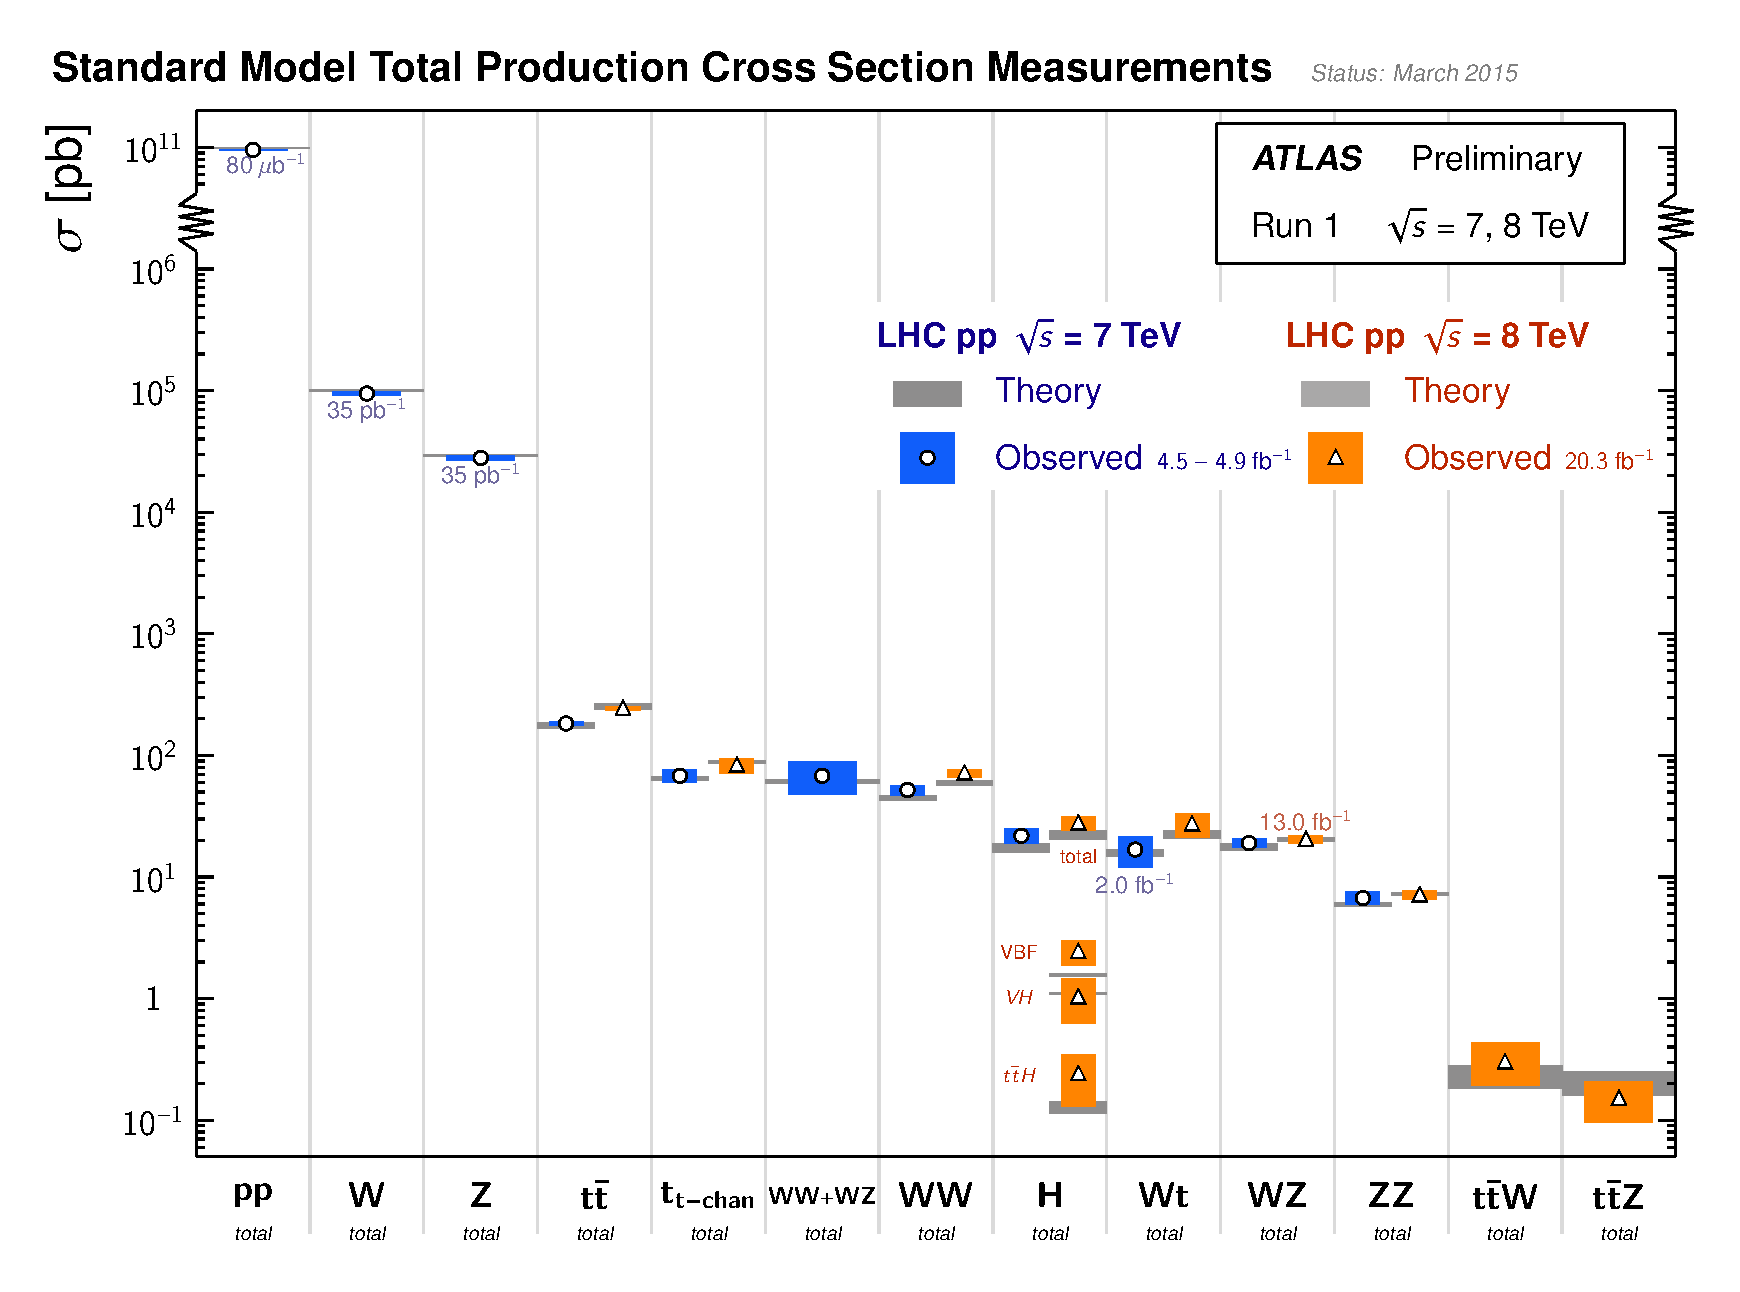
\includegraphics[width=1\textwidth]{figures/ATLAS_a_SMSummary_TotalXsect.pdf}
  \caption{Resumen de las distintas medidas de sección eficaz de producción de
    procesos del SM, comparadas con sus valores teóricos esperados.
    Los valores teóricos esperados fueron calculados como mínimo a NLO\cite{ATLASSM}.}
  \label{fig:sm_atlas_xs}
\end{figure}


\section{Física más allá del SM}

El SM provee una descripción extremadamente exitosa de todos los fenómenos
accesibles con los experimentos de altas energías disponibles actualmente.
Sin embargo,
también se sabe que el SM sufre de algunas debilidades, tanto desde el punto de
vista teórico, como experimental.

El hecho de que existan cuatro tipos de interacciones distintas e independientes
es un poco insatisfactorio y desde Einstein se ha especulado que estas
diferentes interacciones sean distintas manifestaciones de un único campo
unificado. En los a\~nos 1970, los experimentos mostraron que la interacciones
débil y electromagnética podían ser unificadas, motivando aún mas esta idea.
%% La interacción fuerte, aunque
%% esta incluida dentro del SM no esta unificada con las demás, y la interacción
%% gravitatoria ni siquiera forma parte del SM.

Está claro que el SM es una teoría efectiva a bajas energías, muy precisa hasta
escalas de energía del orden de los 100 {\gev}. Sin embargo, los físicos
teóricos creen que el éxito del SM no va a durar a energías mayores. Esta
creencia surge de los intentos de incorporar el SM en una teoría mas
fundamental. Incluso ante la ausencia de la gran unificación de las fuerzas
electrodébil y fuerte a una escala muy alta de energía, el SM tiene que ser
modificado para incorporar los efectos de la gravedad a la escala de Planck.

El SM tiene 25 (ó 26) parámetros libres. Están las masas de los doce fermiones;
las tres constantes de acoplamiento $g$, $g'$ y $g_s$; los dos parámetros que
describen el potencial de Higgs $v$ y $m_H$; y los ocho ángulos de mezcla. Y
además el Lagrangiano de QCD puede contener una fase, $\theta_{\text{CP}}$ que
experimentalmente se conoce que es $\sim 0$. Esta gran cantidad de parámetros
libres se eligen para ajustarse a los datos observados, y no provienen de
principios teóricos más fundamentales, lo cual es otro síntoma de debilidad.

En este contexto también resulta inexplicable por qué el cociente $m_W/m_P \sim
10^{-17}$ es tan chico. A esto se lo conoce como problema de \emph{jerarquía}.
Además, en el SM, la escala de las interacciones electrodébiles se derivan de un
campo escalar elemental que adquiere un valor de expectación de vacío de $v = 2
m_W /g = 246 \gev$. Sin embargo, si uno acopla una teoría de partículas
escalares a nueva física a alguna escala arbitraria $\Lambda$, las correcciones
radiativas al cuadrado de la masa escalar son del orden de $\Lambda^2$, debido a
las divergencias cuadráticas en la auto-energía, lo cual indica la sensibilidad
cuadrática a la mayor escala de energía de la teoría. Por esto, la masa
``natural'' de cualquier partícula escalar es $\Lambda$. Así, para tener una teoría
electrodébil exitosa, la masa del Higgs debe ser del orden de la escala
electrodébil. Este hecho, que la masa del bosón de Higgs no puede ser igual a su
valor natural de $M_P$, es llamado del problema de \emph{naturalidad}.

Desde el punto de vista experimental, también existen algunos resultados que no
pueden acomodarse dentro del SM. El SM considera a los neutrinos como partículas
no masivas, pero distintos
experimentos\cite{PhysRevLett.101.111301,PhysRevD.78.032002} han observado
oscilaciones de sabor en los neutrinos, lo que puede explicarse en el caso en
que estos tengan una masa no nula. Por el momento sólo existen limites
superiores para estas estas masas (ver \cref{tab:fermions}). Los neutrinos
tienen masas muy peque\~nas comparadas con los demás fermiones. El termino de
masa para fermiones puede escribirse usando el doblete de Higgs si existen los
fermiones de helicidad izquierda y derecha para un dado sabor. La masa obtenida
por esta interacción es llamada masa de Dirac. Para que este mecanismo puede ser
utilizado en los neutrinos, deberían existe los neutrinos de helicidad derecha.

El SM tampoco provee un candidato para explicar la naturaleza de la materia
oscura. La existencia de la materia oscura fue inferida por primera vez como
resultado de las inconsistencias observadas entre la masa estimada de las curvas
de rotación galácticas y de su luminosidad\cite{DM1}.
Solo el 4\% del universo consiste en la materia que
conocemos\cite{DM2}. Cerca del 73\% consiste en energía oscura, y el restante
23\% es materia oscura. Como esta materia oscura no interactúa por medio de
interacciones fuerte y electromagnética, y la interacción débil es despreciable
en largas distancias, la materia oscura solo interactúa vía gravedad. La única
partícula del SM que podría ser un candidato viable de materia oscura es el
neutrino, pero como su masa es muy chica para poder explicar estos fenómenos,
puede descartarse.

%% Durante las ultimas décadas se ha intentando solucionar estos problemas.
%% Las soluciones propuestas involucran remover las
%% divergencias cuadráticas de la teoría que son la causa de los problemas de
%% jerarquía y naturalidad. Se han propuesto dos clases de soluciones. En una, los
%% escalares elementales son removidos, y por lo tanto uno debe agregar nuevos
%% fermiones y fuerzas fundamentales. Ejemplos de esto son los modelos de
%% \emph{tecnicolor} o los modelos \emph{compuestos}. La segunda clase de modelos
%% son aquellos en los que se introducen nuevas partículas al SM de forma de
%% cancelar exactamente las divergencias cuadráticas. Esta cancelación solo puede
%% ser el resultado de una nueva simetría.

Son varias las teorías que intentan explicar parcial o totalmente los problemas
mencionados. Estas se conocen como teorías de física mas allá del SM y entre
ellas se encuentra la Supersimetría, modelos con dimensiones extra, teoría de
cuerdas, teorías technicolor, etc. En el siguiente capítulo se explicará brevemente
en qué consiste una de las teorías de física mas allá del SM mas motivadas desde
el punto de vista teórico y experimental, que es la Supersimetría.
